\section{含时微扰}

\begin{quotation}
“人们摆脱不了这种感觉,即这些数学公式有其独立的存在和智能,它们比人更聪明,甚至比它们的发现者还要聪明。人们从方程中所得到的,比最开始所投入的还要多。”\qquad 赫兹
\end{quotation}

为了研究光谱跃迁, 我们需要发展含时微扰(Time-dependent
perturbation)理论. 所谓含时微扰, 就是$H'$是显含时间$t$的, 即$H'(t)$,
总哈密顿量是:

\begin{equation*}
H = H_0 + H'(t)
\end{equation*}

\subsection{相互作用绘景}

态矢量随时间的演化, 部分地是由于$H_0$, 部分地是由于$H'(t)$,
最好能把这两个因素分开. 为此, 我们将使用相互作用绘景(Interaction
picture)\index{Interaction picture: 相互作用绘景}.

在相互作用绘景下, 态矢量$\left| \alpha, t_0 \to t \right\rangle_I$:


\begin{equation*}
\left| \alpha, t_0 \to t \right\rangle_I = e^{iH_0t/\hbar} \left|
\alpha, t_0 \to t \right\rangle_S
\end{equation*}


这里脚标I表示``相互作用绘景'', 脚标S表示``薛定谔绘景''。

相互作用绘景下, 物理量A的期望值是:

\begin{eqnarray*}
% \nonumber to remove numbering (before each equation)
\left\langle A \right\rangle &=& {}_S\left\langle \alpha, t_0, t
\right| A_S \left| \alpha, t_0, t \right\rangle_S \\
  {} &=& {}_S\left\langle \alpha, t_0, t \right|e^{-iH_0t/\hbar}
e^{iH_0t/\hbar} A_S e^{-iH_0t/\hbar} e^{iH_0t/\hbar} \left| \alpha,
t_0, t \right\rangle_S\\
 {} &=& {}_I\left\langle \alpha, t_0,t \right|A_I(t) \left|\alpha, t_0,t  \right\rangle_I
\end{eqnarray*}

算符在相互作用绘景下是:

\begin{equation*}
A_I(t)=e^{iH_0t/\hbar} A_S e^{-iH_0t/\hbar}
\end{equation*}

对态矢量$\left| \alpha,t_0,t  \right\rangle_I $,
我们来计算它随时间的演化.

\begin{eqnarray*}
% \nonumber to remove numbering (before each equation)
i\hbar \frac{\partial}{\partial t} \left| \alpha,t_0,t  \right\rangle_I &=& i\hbar \frac{\partial}{\partial t} \left( e^{iH_0t/\hbar} \left| \alpha,t_0,t  \right\rangle_S \right)  \\
  {} &=& -H_0e^{iH_0t/\hbar}\left|\alpha, t_0,t \right\rangle_S + e^{iH_0t/\hbar} H \left|\alpha, t_0,t
  \right\rangle_S\\
  {} &=& e^{iH_0t/\hbar}(H-H_0)e^{-iH_0t/\hbar}e^{iH_0t/\hbar}\left|\alpha, t_0,t
  \right\rangle_S\\
  {} &=& e^{iH_0t/\hbar}H'e^{-iH_0t/\hbar}e^{iH_0t/\hbar}\left|\alpha, t_0,t
  \right\rangle_S\\
  {} &=& H'_I(t)\left|\alpha, t_0,t
  \right\rangle_I
\end{eqnarray*}

即:

\begin{equation*}
i\hbar \frac{\partial}{\partial t} \left| \alpha,t_0,t
\right\rangle_I = H'_I(t)\left|\alpha, t_0,t \right\rangle_I.
\end{equation*}

这个式子也叫做薛定谔方程, 它决定了态矢随时间演化的规律,
在相互作用绘景下, 它将只由``相互作用''$H'_I$决定.

此外, 我们还可以推出算符随时间演化的规律,
即相互作用绘景下的海森堡运动方程:


\begin{equation*}
    i\hbar \frac{dA_I}{dt} = [A_I, H_0]
\end{equation*}

即算符随时间的演化将完全由$H_0$决定.

\subsection{含时微扰}


假设$\{ \left|n \right\rangle \}$是相互作用绘景下的基态, $\left|
\alpha, t_0,t \right\rangle_I$可以用$\{ \left|n \right\rangle
\}$展开:


\begin{equation*}
\left| \alpha, t_0,t \right\rangle_I = \sum_n c_n (t) \left|n
\right\rangle
\end{equation*}

左右两边左乘$\left\langle n \right|$, 得到关于$c_n(t)$的微分方程:


\begin{equation*}
i \hbar \frac{\partial}{\partial t} \left\langle n | \alpha,
t_0,t\right\rangle_I = \sum\limits_m \left\langle n \right| H'_I
\left|m \right\rangle \left\langle m | \alpha, t_0,t \right\rangle_I
\end{equation*}

这里矩阵元$\left\langle n \right| H'_I \left|m \right\rangle$是:

\begin{equation*}
\left\langle n \right| e^{iH_0t/\hbar}H'e^{-iH_0t/\hbar}\left|m
\right\rangle = H'_{nm} e^{i (E_n -E_m)t/\hbar}
\end{equation*}

定义: $E_n - E_m = \hbar \omega_{nm}$, 则微分方程可写为:

\begin{equation*}
i\hbar \frac{d}{dt} c_n(t) = \sum\limits_{m}
H'_{nm}e^{i\omega_{nm}t}c_m(t)
\end{equation*}

改写成矩阵的形式:


\begin{equation}\label{time dependent sch eq matrix}
i\hbar \left( \begin{array}{l}
 \dot c_1  \\
 \dot c_2  \\
 ... \\
 \end{array} \right) = \left( {\begin{array}{*{20}c}
   {H'_{11} } & {H'_{12} e^{i\omega _{12} t} } & {...}  \\
   {H'_{21} e^{i\omega _{21} t} } & {H'_{22} } & {...}  \\
   {...} & {...} & {...}  \\
\end{array}} \right)\left( \begin{array}{l}
 c_1  \\
 c_2  \\
 ... \\
 \end{array} \right)
\end{equation}

\subsubsection*{含时双态问题}


大部分含时问题没有严格解, 但含时双态问题(Time-dependent two-state
problem)存在严格解。核磁共振(Nuclear magnetic resonance, NMR),
自旋磁共振(Spin magnetic resonance)和微波激射(Maser)等都属于含时双态问题, 哈密顿可写为:

\index{Nuclear magnetic resonance, NMR: 核磁共振}

\begin{eqnarray*}
% \nonumber to remove numbering (before each equation)
  H_0 &=& E_1 | 1 \rangle \langle 1| + E_2 | 2 \rangle \langle 2| \\
  H'(t) &=& \gamma e^{i \omega t} | 1 \rangle \langle 2 | + \gamma
e^{- i \omega t} | 2 \rangle \langle 1 |
\end{eqnarray*}

需求解二元一阶微分方程组, 假设初始条件$c_1(0) =1$, $c_2(0)=0$,
我们将得到著名的拉比公式(Rabi's formula)\index{Rabi's formula: 拉比公式},

\begin{eqnarray*}
% \nonumber to remove numbering (before each equation)
  \left| {c_1 \left( t \right)} \right|^2 &=& \cos ^2 \Omega t +
\frac{{\left( {{\textstyle{{\omega  - \omega _{21} } \over 2}}}
\right)^2 }}{{\Omega ^2 }}\sin ^2 \Omega t \\
  \left| {c_2 \left( t
\right)} \right|^2 &=& \frac{{\left( {{\textstyle{\gamma  \over
\hbar }}} \right)^2 \sin ^2 \Omega t}}{{\Omega ^2 }}
\end{eqnarray*}


这里, $\Omega  = \sqrt {\left( {\frac{\gamma }{\hbar }} \right)^2  +
\left( {\frac{{\omega  - \omega _{21} }}{2}} \right)^2 } $,
满足:$\left| {c_1 \left( t \right)} \right|^2  + \left| {c_2 \left(
t \right)} \right|^2  = 1$。说明系统将在$1$态和$2$态之间振荡。



\subsubsection*{迭代求解}

对方程(\ref{time dependent sch eq matrix}), 我们可用迭代的方法求解,
假设波函数$c_n(t)$可写成微扰展开的形式: $c_n(t) = c_n^{(0)} +
c_n^{(1)} + c_n^{(2)} + ...$


假设$t=0$时, 系统处在某特定的$\left| i \right\rangle $态上, 则:
$c_n^{(0)} = \delta_{ni}$,
把这个作为0阶近似代入含时薛定谔方程(\ref{time dependent sch eq
matrix})中, 我们将得到1阶近似: $c_n^{(1)}$,
再代入则得到$c_n^{(2)}$等等。

\begin{description}
  \item[$0$阶] $c_n^{(0)} (t) = \delta_{ni}$
  \item[$1$阶] $c_n^{(1)}(t) = \frac{1}{i\hbar} \int_{t_0}^t dt' e^{i \omega_{ni}
t'}H'_{ni}(t')$
  \item[$2$阶] $c_n^{(2)}(t) = (\frac{1}{i\hbar})^2 \sum\limits_m \int_{t_0}^t dt'
\int_{t_0}^{t'} dt'' e^{i
\omega_{nm}t'}H'_{nm}(t')e^{i\omega_{mi}t''}H'_{mi}(t'')$
\end{description}


那么$ i \to n$($i \ne n$)的跃迁几率为\footnote{J J Sakurai, Modern
Quantum Mechanics, pp328}:


\begin{equation*}
P(i \to n)=|c_n^{(1)}(t) + c_n^{(2)}(t) + ... |^2
\end{equation*}


\subsection{常微扰}

\begin{center}
$H'(t) = \left\{ \begin{array}{l}
 H',t \in \left[ {0,T} \right] \\
 0,{\rm{others}} \\
 \end{array} \right.$
\end{center}


解:$t > T$时,

$\begin{array}{l}
 a_m^{(1)} (t) = \frac{1}{{i\hbar }}\int_0^t {dt'H'_{mk} (t'){\mathop{\rm e}\nolimits} ^{i\omega _{mk} t'} }  = \frac{{H'_{mk} }}{{i\hbar }}\int_0^t {dt'{\mathop{\rm e}\nolimits} ^{i\omega _{mk} t'} }  \\
  = \frac{{H'_{mk} }}{{i\hbar }}\left[ {\frac{{{\mathop{\rm e}\nolimits} ^{i\omega _{mk} t'} }}{{i\omega _{mk} }}} \right]_0^t  = \frac{{H'_{mk} }}{{i\hbar }}\frac{{{\mathop{\rm e}\nolimits} ^{i\omega _{mk} T}  - 1}}{{i\omega _{mk} }} = \frac{{H'_{mk} }}{{\hbar \omega _{mk} }}\left( {1 - {\mathop{\rm e}\nolimits} ^{i\omega _{mk} T} } \right) \\
 \end{array}$

跃迁几率:

$\begin{array}{l}
 W_{k \to m}  = \left| {\frac{{H'_{mk} }}{{\hbar \omega _{mk} }}} \right|^2  \cdot \left| {1 - e^{i\omega _{mk} T} } \right|^2   \\
 = \left| {\frac{{H'_{mk} }}{{\hbar \omega _{mk} }}} \right|^2 \left( {1 - \cos \omega T - i\sin \omega T} \right)\left( {1 - \cos \omega T + i\sin \omega T} \right) \\
 = \left| {\frac{{H'_{mk} }}{{\hbar \omega _{mk} }}} \right|^2 \left( {2 - 2\cos \omega T} \right) = \left| {\frac{{H'_{mk} }}{{\hbar \omega _{mk} }}} \right|^2 2 \cdot 2\sin ^2 {\textstyle{{\omega T} \over 2}} \\
 = \left| {\frac{{H'_{mk} }}{\hbar }} \right|^2 \frac{{\sin ^2 {\textstyle{{\omega _{mk} T} \over 2}}}}{{\left( {{\textstyle{{\omega _{mk} } \over 2}}} \right)^2 }} \\
 \end{array}$

显然有:$W_{km}  = W_{mk} $


\begin{figure}[h]
\begin{center}
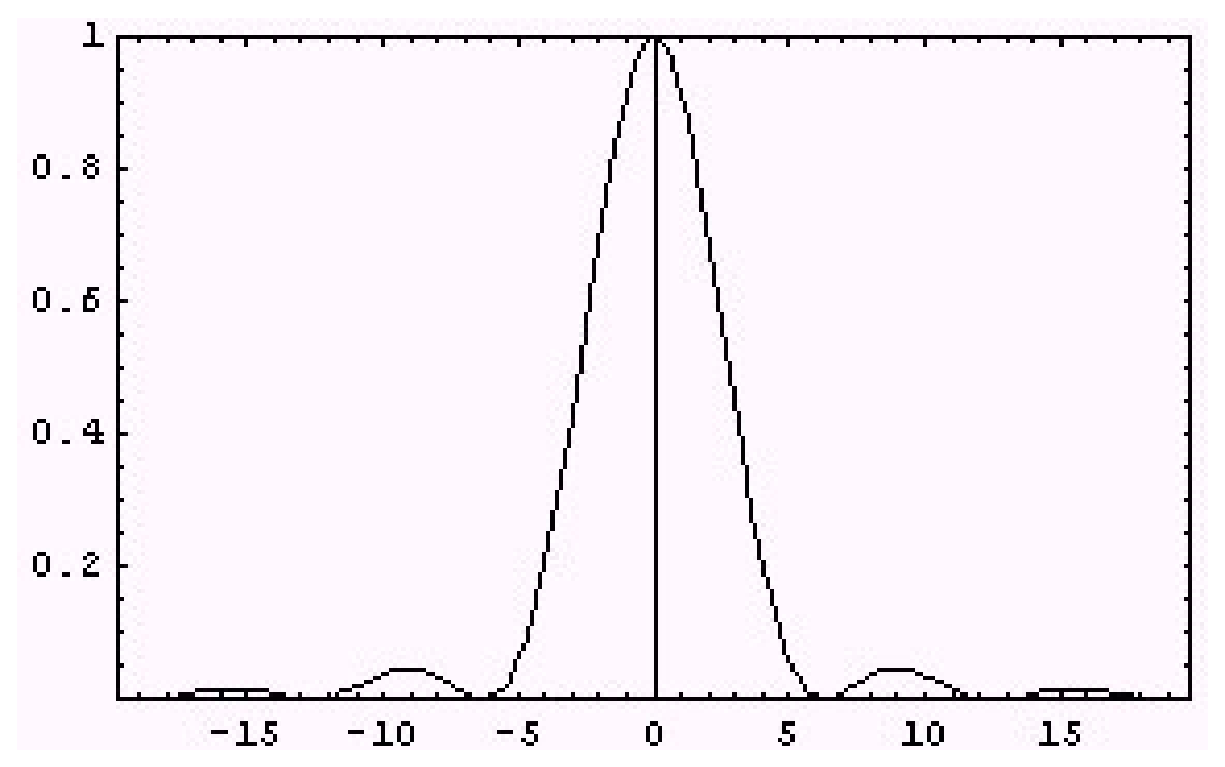
\includegraphics[clip,width=7cm]{Perturbation/ConstantPerturbation.ps}
\caption{跃迁几率函数$\frac{{\sin ^2 {\textstyle{{\omega _{mk} T}
\over 2}}}}{{\left( {{\textstyle{{\omega _{mk} } \over 2}}}
\right)^2 }}$}
\end{center}
\end{figure}

利用$\delta$函数:$\mathop {\lim }\limits_{\alpha  \to \infty }
\frac{{\sin ^2 \alpha x}}{{x^2 }} \to \pi \alpha \delta (x)$


\begin{equation}\label{24-18}
\mathop {\lim }\limits_{T \to \infty } \frac{{\sin ^2
{\textstyle{{\omega _{mk} T} \over 2}}}}{{\left(
{{\textstyle{{\omega _{mk} } \over 2}}} \right)^2 }} \to \pi T\delta
\left( {{\textstyle{{\omega _{mk} } \over 2}}} \right) = 2\pi
T\delta (\omega _{mk} )
\end{equation}

所以:$W_{k \to m}  = 2\pi T\left| {\frac{{H'_{mk} }}{\hbar }}
\right|^2 \delta (\omega _{mk} )$

跃迁速率为:

\begin{equation}\label{24-19}
w_{k \to m}  = \frac{{W_{k \to m} }}{T} = \frac{{2\pi }}{{\hbar ^2
}}\left| {H'_{mk} } \right|^2 \delta (\omega _{mk} ) = \frac{{2\pi
}}{\hbar }\left| {H'_{mk} } \right|^2 \delta (E_m  - E_k )
\end{equation}

\textbf{Fermi黄金规则(Golden Rule):}假设末态($m$态)是连续变化情况,$m$态附近态密度为:$\rho(E_m)$,则从初态($k$态)演化到$m$态附近所有可能末态的跃迁速率之和是:


\begin{equation}\label{24-20}
w_{km}  = \int {\frac{{2\pi }}{\hbar }\left| {H'_{mk} } \right|^2
\rho (E_m )\delta (E_m  - E_k )} dE_m  = \frac{{2\pi }}{\hbar
}\left| {H'_{mk} } \right|^2 \rho (E_m )
\end{equation}


\subsection{简谐微扰}

就是$\sin$, $\cos$型的微扰, 假设微扰是:

\begin{equation}\label{Harmonic Perturbation}
V(t)= 2 V_0 \cos \omega t = V_0 \left( e^{i \omega t} + e^{- i
\omega t} \right)
\end{equation}


假设系统起初都处于$i$态, 然后自$t=0$起, $V(t)$起作用, 当$t = t$时,
一阶含时微扰:

\begin{eqnarray*}
% \nonumber to remove numbering (before each equation)
  c_n &=& \frac{1}{i \hbar} \int_0^t V_0 \left( e^{i \omega t'} + e^{-i \omega t'}  \right) e^{i \omega_{ni}} t' d t' \\
  {} &=& \frac{V_0}{\hbar} \left( \frac{1-e^{i(\omega_{ni} + \omega)t}}{\omega_{ni} + \omega }  + \frac{1-e^{i(\omega_{ni} - \omega)t}}{\omega_{ni} - \omega} \right)
\end{eqnarray*}

当$t \to \infty$时,

(1)当$\omega_{ni} + \omega \to 0$, 即: $E_n \approx E_i - \hbar
\omega $, 对应辐射过程, 或:

(2)当$\omega_{ni} - \omega \to 0$, 即:$E_n \approx E_i + \hbar
\omega$, 对应吸收过程.

这些过程的发生是以$V(t)$微扰为前提的, 因此前者是受激辐射(stimulated
emission)\index{Stimulated emission: 受激辐射}, 后者是受激吸收(stimulated absorption)\index{Stimulated absorption: 受激吸收}.


模仿常微扰, 我们可以写出跃迁速率:


\begin{eqnarray*}
% \nonumber to remove numbering (before each equation)
  w_{i \to n} &=& \frac{2\pi}{\hbar} \overline{|V_0|^2} \rho (E_n) |_{E_n \approx E_i - \hbar \omega} \\
  w_{i \to n} &=& \frac{2\pi}{\hbar} \overline{|V_0|^2} \rho (E_n) |_{E_n \approx E_i + \hbar \omega}
\end{eqnarray*}

对吸收过程,做个改写:

\begin{equation*}
    w_{n \to i} = \frac{2\pi}{\hbar} \overline{|V_0|^2} \rho (E_i) |_{E_i \approx E_n + \hbar \omega}
\end{equation*}


得到细致平衡(detailed balancing)\index{Detailed balancing: 细致平衡}条件:

\begin{equation}\label{detailed balancing}
 \frac{w_{i \to n}}{\rho (E_n) } = \frac{w_{n \to i}}{\rho (E_i)}
\end{equation}


\subsection*{阅读与思考}

推荐阅读:查尔斯·汤斯,《创造波浪——从微波激射器到我的科学观》